% !TeX program = xelatex
% 將 git_commands.png 放在本檔同一資料夾；使用 XeLaTeX 編譯兩次。
\documentclass[UTF8,fontset=fandol,11pt,a4paper]{ctexart}
\usepackage[margin=2.2cm]{geometry}
\usepackage{graphicx,xcolor,booktabs,tabularx,fancyvrb,enumitem}
\usepackage[unicode,colorlinks=true,linkcolor=blue!50!black,urlcolor=blue!60!black]{hyperref}
% Windows 若偏好標楷體，可取消下一行註解：
\setCJKmainfont{標楷體}
\setlength{\parindent}{0pt}
\setlength{\parskip}{6pt}
\DefineVerbatimEnvironment{code}{Verbatim}{fontsize=\small,frame=single,framesep=3mm}
\title{Git 基礎教學\\\large 從建立版本庫到 GitHub 同步}
\author{}
\date{}
\begin{document}
\maketitle
\textbf{核心流程：修改檔案 → git add → git commit → git push。}
\tableofcontents
\newpage
\section{Git 到底在做什麼？}
Git 是分散式版本控制系統，可記錄專案每一次提交的狀態，讓你查閱修改、比較版本、建立分支，或恢復先前內容。例如筆記先完成 Euler--Lagrange 方程，再補上例題，每個完成階段都能留下獨立版本。多數本機操作不需要網路。
\section{Git 與 GitHub 的差別}
\begin{tabularx}{\linewidth}{lXX}\toprule
       & Git         & GitHub         \\\midrule
    性質 & 版本控制工具      & 遠端 Git 版本庫託管平台 \\
    用途 & 提交、比較、分支、合併 & 分享、協作、異地保存版本   \\
    位置 & 可在自己的電腦操作   & 網路服務           \\\bottomrule
\end{tabularx}
\section{三個區域與遠端版本庫}
\begin{description}[leftmargin=2cm]
    \item[工作目錄] 實際編輯檔案的地方（working directory／workspace）。
    \item[暫存區] 準備在下一次提交收錄的內容（staging area／index）。
    \item[本地版本庫] 已經提交的版本紀錄（local repository）。
    \item[遠端版本庫] 透過網路同步的 Git 版本庫（remote repository）。
\end{description}
\texttt{git add} 選擇修改；\texttt{git commit} 建立本地版本；\texttt{git push} 上傳提交。
\section{Git 指令流程圖}
\begin{figure}[htbp]
    \centering
    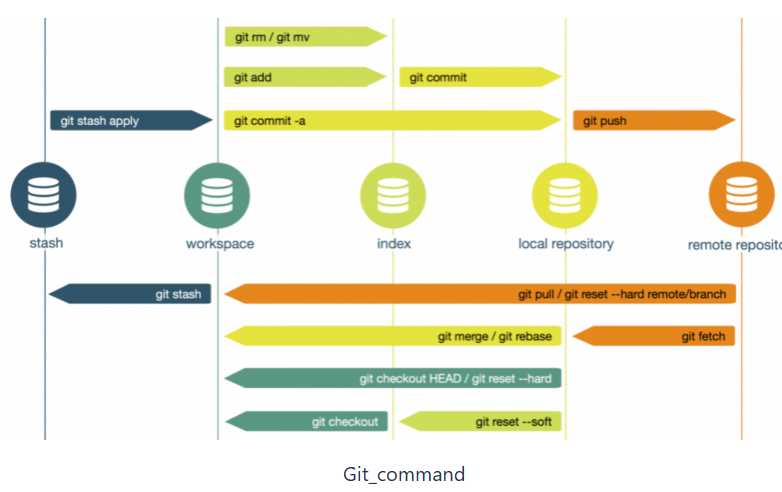
\includegraphics[width=\linewidth]{git_commands.png}
    \caption{使用者提供的 Git 指令流程圖。}
\end{figure}
讀圖時先找 workspace、index、local repository、remote repository 四個位置，再看箭頭上的指令。stash 是暫時收起未完成修改的地方。
\begin{itemize}
    \item \texttt{git commit -a} 自動暫存已追蹤檔案的修改與刪除，\textbf{不會加入尚未追蹤的新檔案}。
    \item \texttt{git fetch} 取得遠端資料並更新遠端追蹤分支，不直接合併進目前分支。
    \item \texttt{git pull} 先取得遠端資料，再依選項或設定進行合併或 rebase。
    \item 圖中 \texttt{checkout} 涵蓋多種舊式用法；初學可用 \texttt{switch} 切分支、\texttt{restore} 恢復檔案。
    \item \texttt{reset --hard} 可能捨棄已追蹤檔案尚未提交的修改，不能當成一般同步指令。
\end{itemize}
\section{第一次使用 Git}
先確認安裝，設定未來提交所記錄的作者姓名與電子郵件：
\begin{code}
    git --version
    git config --global user.name "Chen-An"
    git config --global user.email "example@gmail.com"
    git config --list
\end{code}
請把範例姓名與 Email 換成自己的資料。這是提交作者資訊，不是 GitHub 登入設定。
\section{建立本地版本庫：git init}
\begin{code}
    mkdir physics-project
    cd physics-project
    git init -b main
\end{code}
Git 會建立隱藏的 \texttt{.git} 資料夾，保存歷史與設定，請勿任意刪除。已經是版本庫的專案不需要反覆初始化。
\section{查看狀態：git status}
\begin{code}
    git status
\end{code}
\texttt{Untracked files} 表示尚未追蹤的新檔案；\texttt{Changes not staged for commit} 是尚未暫存的修改；\texttt{Changes to be committed} 是下次提交將收錄的內容。
\section{加入暫存區：git add}
\begin{code}
    git add main.py
    git add .
\end{code}
第一行加入指定檔案；第二行暫存目前目錄及子目錄的變更（忽略規則仍適用）。\texttt{add} 收錄的是當下內容，若之後再修改檔案，要再執行一次 \texttt{add} 才會納入新的修改。
\section{建立版本：git commit}
\begin{code}
    git commit -m "完成牛頓運動模擬"
\end{code}
提交一般只收錄暫存區內容。訊息用一句話說明本次完成的工作，例如「補上簡諧振子解析解」或「修正球座標 Jacobian 推導」。
\section{add 與 commit 差在哪？}
假設同時修改 \texttt{main.py}、\texttt{plot.py} 與 \texttt{README.md}，這次只要提交程式變更：
\begin{code}
    git add main.py plot.py
    git commit -m "加入繪圖功能"
\end{code}
README 的尚未暫存修改仍留在工作目錄。\textbf{add 是選擇內容，commit 是正式建立版本。}
\section{日常工作循環}
\begin{code}
    git status
    git diff
    git add .
    git diff --staged
    git commit -m "加入簡諧振子模型"
\end{code}
每完成一段有意義的工作就提交，方便日後查詢與恢復。提交前檢查暫存區，可避免把無關內容一起收錄。
\section{查看歷史：git log}
\begin{code}
    git log
    git log --oneline
    git log --oneline --graph --all
\end{code}
\texttt{--oneline} 每個提交顯示一行；\texttt{--graph --all} 可觀察各分支的歷史。若進入分頁畫面，按 \texttt{q} 離開。
\section{比較修改：git diff}
\begin{code}
    git diff
    git diff --staged
\end{code}
第一行比較工作目錄與暫存區；第二行比較暫存區與目前提交。差異中的減號表示刪除的行，加號表示新增的行。未追蹤新檔案通常不會出現在一般 \texttt{git diff} 中。
\section{在 GitHub 建立遠端版本庫}
在 GitHub 建立新 repository。若要推送已存在的本地專案，練習時可先建立空的遠端版本庫，避免兩邊各有不同初始提交。複製該版本庫 URL，並依 GitHub 提示完成驗證。
\section{加入遠端位置：git remote}
\begin{code}
    git remote add origin https://github.com/username/physics-project.git
    git remote -v
\end{code}
請替換成自己的 URL。\texttt{origin} 是遠端名稱的慣例，不是 GitHub 的固定代稱；遠端也可以是其他服務。
\section{上傳提交：git push}
\begin{code}
    git push -u origin main
\end{code}
第一次使用 \texttt{-u} 設定本地分支的上游。之後在此分支通常可以直接：
\begin{code}
    git push
\end{code}
推送上傳已提交的版本，尚未提交的工作目錄修改不會跟著上傳。
\section{取得既有專案：git clone}
\begin{code}
    git clone https://github.com/username/physics-project.git
    cd physics-project
\end{code}
一般 clone 會取得專案與歷史、建立本地版本庫並設定 origin。\texttt{init} 適合建立新本地專案，\texttt{clone} 適合取得既有遠端專案。
\section{取得並整合遠端更新：git pull}
\begin{code}
    git status
    git pull --ff-only
\end{code}
先確認自己的工作已妥善保存。\texttt{--ff-only} 只允許快轉；若本地與遠端已各自新增提交，就會停止，讓你先了解差異再決定如何合併。一般 \texttt{git pull} 的整合方式受選項與設定影響。
\section{建立與切換分支}
分支適合用來試作新功能，例如嘗試新的數值模擬方法：
\begin{code}
    git branch
    git switch -c feature-simulation
\end{code}
\texttt{switch -c} 同時建立與切換分支。若分支已存在：
\begin{code}
    git switch feature-simulation
\end{code}
舊教材的 \texttt{git checkout -b} 也能建立並切換分支。分支共享工作目錄，切換前應先提交或暫存未完成的修改。
\section{合併分支：git merge}
功能完成並提交後，切回要接收變更的分支，再合併：
\begin{code}
    git switch main
    git merge feature-simulation
\end{code}
合併可能是快轉，也可能建立合併提交。若發生衝突，編輯衝突檔案、確認內容後 \texttt{git add}，再 \texttt{git commit}。若需要中止尚未完成的合併：
\begin{code}
    git merge --abort
\end{code}
\section{暫時收起工作：git stash}
\begin{code}
    git stash push -u -m "模擬功能進行中"
    git stash list
    git stash pop
\end{code}
\texttt{-u} 同時收起未追蹤檔案；一般 stash 不包含未追蹤檔案或被忽略的檔案。\texttt{pop} 套用成功後移除該筆 stash；若有衝突，該筆通常會保留，需自行處理。\texttt{git stash apply} 則套用但保留該筆紀錄。
\section{忽略暫存檔：.gitignore}
在專案根目錄建立 \texttt{.gitignore}，範例適合 Python 與 LaTeX：
\begin{code}
    # Python
    __pycache__/
    .venv/
    # LaTeX
    *.aux
    *.log
    *.out
    *.toc
    *.synctex.gz
    *.fls
    *.fdb_latexmk
\end{code}
保留 \texttt{.tex} 與必要圖片；PDF 是否追蹤可依用途決定。忽略規則不會自動停止追蹤已經提交的檔案。\texttt{.gitignore} 本身也應提交。
\section{安全的恢復方式}
取消某檔案的暫存，但保留工作目錄修改（已有提交時）：
\begin{code}
    git restore --staged main.py
\end{code}
捨棄該檔案尚未暫存的修改，還原成暫存區內容：
\begin{code}
    git restore main.py
\end{code}
第二個指令會覆蓋未暫存內容，執行前先確認差異。若要撤銷已提交的某次變更並留下撤銷紀錄，可用 \texttt{git revert}，例如：
\begin{code}
    git revert HEAD
\end{code}
初學不需要先背 \texttt{reset --hard} 或強制推送。
\section{常用指令速查表}
\begin{tabularx}{\linewidth}{lX}\toprule
    指令                           & 功能           \\\midrule
    \texttt{git init -b main}    & 建立本地版本庫      \\
    \texttt{git clone URL}       & 取得遠端專案       \\
    \texttt{git status}          & 查看工作與暫存狀態    \\
    \texttt{git add .}           & 暫存目前目錄的變更    \\
    \texttt{git commit -m "..."} & 建立版本         \\
    \texttt{git log --oneline}   & 查看提交紀錄       \\
    \texttt{git diff}            & 查看尚未暫存的修改    \\
    \texttt{git diff --staged}   & 查看將提交的修改     \\
    \texttt{git pull --ff-only}  & 取得更新並嘗試快轉    \\
    \texttt{git push}            & 推送已提交版本      \\
    \texttt{git switch -c NAME}  & 建立並切換分支      \\
    \texttt{git merge NAME}      & 合併指定分支至目前分支  \\
    \texttt{git stash push -u}   & 暫時收起工作與未追蹤檔案 \\\bottomrule
\end{tabularx}
\section{實際練習：建立兩個版本}
\begin{enumerate}
    \item 建立測試專案：
          \begin{code}
              mkdir git-practice
              cd git-practice
              git init -b main
          \end{code}
    \item 用文字編輯器建立 \texttt{hello.txt}，內容為 \texttt{Hello Git}，儲存後執行：
          \begin{code}
              git status
              git add hello.txt
              git status
              git commit -m "建立 hello.txt"
          \end{code}
    \item 在檔案第二行加入 \texttt{My second version}，儲存後執行：
          \begin{code}
              git diff
              git add hello.txt
              git diff --staged
              git commit -m "修改 hello.txt"
              git log --oneline
          \end{code}
\end{enumerate}
你應該看到兩筆提交，較新的提交在上方。接著可試著新增分支、修改檔案並提交，再合併回 main。
\section{套用到 LaTeX 學習筆記}
把主 \texttt{.tex}、必要圖片、參考文獻及 \texttt{.gitignore} 放入同一專案。每次完成一段推導或補上一個例題：
\begin{code}
    git status
    git diff
    git add .
    git diff --staged
    git commit -m "補上第二變分 Hessian 的例題"
    git push
\end{code}
最後一行需先設定遠端與上游。記住：\textbf{選擇修改 → 建立版本 → 上傳版本。}
\section*{參考與編譯說明}
本教學整理自前述對話與使用者指定文章：\\
\url{https://www.maxlist.xyz/post/git_tutorial/}

附圖為使用者提供。使用 XeLaTeX 編譯本檔兩次以更新目錄。預設使用 TeX Live 的 Fandol 字型；Windows 若想使用標楷體，可取消原始碼中 \texttt{DFKai-SB} 設定的註解。
\end{document}
